% lsystems.tex

\marginnote{beginning of models/lsystems.tex}

To motivate our discussion of curve grammars, we will first give an
amusing example of such a grammar, which is inspired by L-systems. A
Lindenmayer system, or L-system, is a parallel string rewriting
system. 
\marginnote{They are intended to be pictures! Cite Lindenmayer's famous book.}
Although they are defined on strings, it is popular to render
their output as a picture using a ``turtle language'' akin to
Logo. They are a simple and intuitive way to generate fractal
images. Since our formalisms do not match up perfectly with the usual
definition of L-systems, we will not discuss them.

We will informally discuss curve rewriting systems, where we
iteratively replace straight lines with curves composed of straight
lines. We will represent our curves like this: \spk{10}{gline}, so that
we remember which endpoint is which.

Consider the following system\footnote{generated by $A=A+A+A--$ with
  angle $60^\circ$ in Inkscape}:
$$ \spk{10}{gline} \to \spk{10}{gbump} .$$

Applying this rule a few times, we generate \spk{10}{gline}, \spk{10}{gbump},
\spk{10}{gbump2} and \spk{15}{gbump3}.

%% An L-system might represent
%% this rewrite rule as $A\to A+A+A$. Here, if we interpret the symbol
%% $A$ as ``go forward one step'' and the symbol $+$ as ``rotate 60
%% degrees to the left'', then a turtle following the directions $A+A+A$
%% would generate the curve 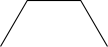
\includegraphics[width=10mm]{bump.png},
%% suitably rotated.

We now wish to construct a more complicated system. We need to start
distinguishing different kinds of curves, in this case \spk{10}{gdash}
versus \spk{10}{gline}. Consider the following system\footnote{generated by 
$A=B+A+B; B=A-B-A$ with angle $60^\circ$ in Inkscape}
\begin{align*}
\spk{15}{gline} &\to \spk{15}{gBAB} \\
\spk{15}{gdash} &\to \spk{15}{gABA}.
\end{align*}

\marginnote{We should put the things on a commons scale.}
If we start from \spk{10}{gline}, we successively generate
\spk{10}{gBAB}, \spk{20}{gsier2}, and \spk{20}{gsier3}.  Suprisingly,
after a large number of iterations, a pattern arises that may be
familiar: Sierpinski's triangle! After eight iterations, we have
(filling in the dashed lines for simplicity) curve $C$:

\spk{100}{gsier8}.

These curves were generated by Inkscape's L-system function, which has
a randomizing option. It is interesting to randomize the last
example. Here is the randomized version $C'$ I got, with fairly little
noise (10\% randomization in the length of line segments, and 5\%
randomization in the angles. These parameters only make sense in a
more standard L-system framework):

\spk{100}{gbadsier}.


\footnote{This is exactly the issue shape-tree addresses in contrast
  to other deformable models.}  This has no global similarity at all
to the other curve! Inkscape is using a Markov-like source of
randomness, and little errors at the local level add up to huge
changes at the global level. If we are going to have a statistical
model for perceptual similarity of curves, we will have to find a way
to introduce long-range dependencies. This brings us to our next
section: probabilistic context-free grammars on curves.

\marginnote{end of models/lsystems.tex}
